\section{Design}

\subsection{Engine}

\subsection{Game System/GUI}


\begin{figure}[htbp]
	\centering
		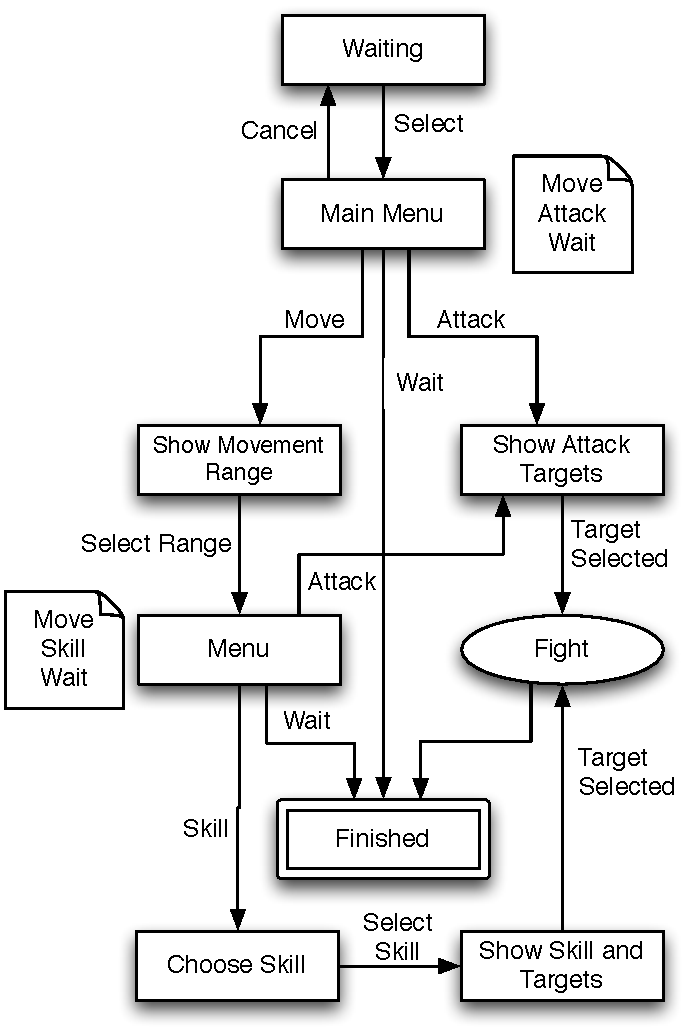
\includegraphics[width=4in]{figures/unit.pdf}
	\caption{The State diagram of a single turn of a player's unit}
	\label{fig:figures_unit}
\end{figure}


\subsection{Editor}

\subsubsection{Exporting}

The editor can export a project as a complete package, either as a Mac OS X application or as jar. These application don't requires any external resources, apart from a recent version of java \footnote{specifically Java 1.6+}.

A notable feature of the editor is that jar will work on any java enabled platform, since the jar contains all required libraries for each platform. The OS X application can even be export on other platforms.

While most of the testing was done on OS X \footnote{Mac OS X 10.6 Snow leopard}, it also works well on Linux \footnote{Science  Linux x.y}. It even has limited compatibly with Windows\footnote{Tested on Windows 7 32 bit} (apart from some minor graphics issues).